Se ingresa el identificador a ser buscado.
\subsection{Subpaso 1-A: Buscar }
\begin{enumerate}
	\item Ingrese identificador.
	\item Presione el botón \textbf{Buscar}. Este paso puede derivar
		al error \textbf{Error E1-A}.

\end{enumerate}

\begin{figure}[hbtp]
		\centering
		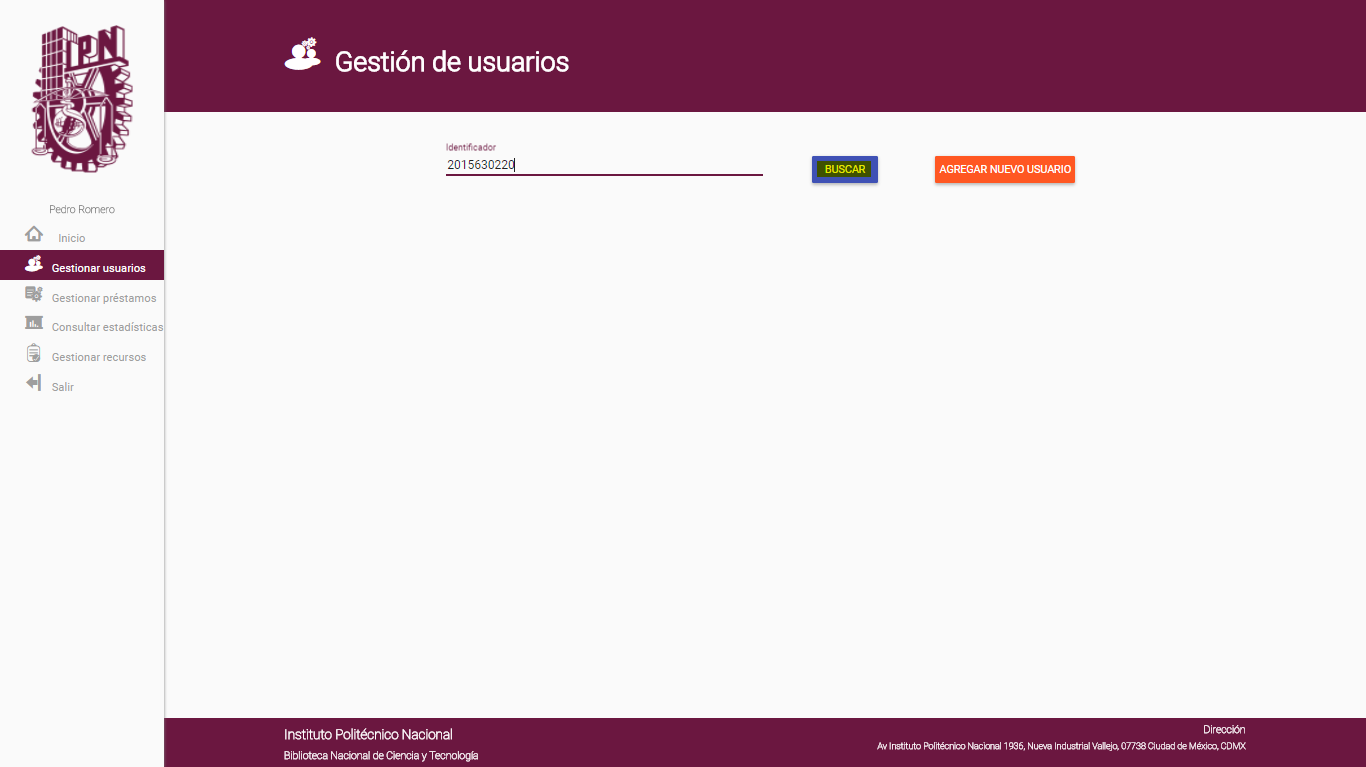
\includegraphics[scale=0.3]{images/Interfaz/IUGS22_gestionarUsuarioBuscar.png}
		\caption{Gestionar Usuario}
	\end{figure}

\subsection{Error E1-A: usuario no encontrado}
El identificador que se ingresó no se encuentra  en el sistema,
debe verificarlo.
\begin{itemize}
	\item Presionar \textbf{Aceptar} en la ventana emergente 
		\textbf{MAT-48 Usuario no encontrado}
		%\begin{figure}[hbtp]
		
		%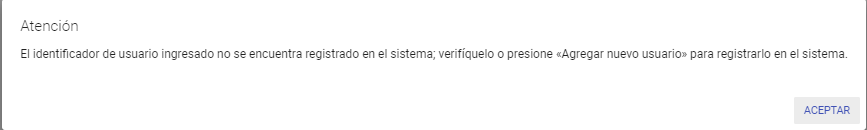
\includegraphics[scale=0.3]{images/Interfaz/MAT48_usuarioNoEncontrado.png}
		%\caption{Gestionar Usuario}
	%\end{figure} 

  %%
  %% Ruta a imagen que no existe.
  %% Cuidado con este tipo de cosas.
  %% RQF7
  %%

\end{itemize}
